\section{Introduction}\label{sec:introduction}

\subsection{The result}\label{subsec:result}

Let $\psi=\Gamma'/\Gamma$ be the digamma function and $\trig=\psi'$ the trigamma function, so
that $\trig(x)=\sum_{j\ge0}(j+x)^{-2}$ for $x>0$. Since $\trig(1/2)=\pi^2/2$
\cite[5.15.3]{DLMF}, the numbers
\begin{equation}\label{eq:xi-def}
  \xi_k:=\trig\!\left(\tfrac k5\right)-\frac{\pi^2}{2}
       =\trig\!\left(\tfrac k5\right)-\trig\!\left(\tfrac12\right),\qquad k=1,2,3,4,
\end{equation}
are differences of trigamma values at a fifth and at one half. Equivalently
$\xi_k=\sum_{n\ge1}a_k(n)n^{-2}$ with $a_k(n)=25\cdot\mathbf 1[n\equiv k\bmod 5]-3$. Numerically
$\xi_1=21.3325750\ldots$, $\xi_2=2.3405543\ldots$, $\xi_3=-1.2985925\ldots$ and
$\xi_4=-2.6353280\ldots$.

\begin{theorem}\label{thm:main}
For each $k\in\{1,2,3,4\}$ the number $\xi_k=\trig(k/5)-\pi^2/2$ is irrational.
\end{theorem}

\Cref{thm:main} is a \emph{candidate} result. Its proof is complete on paper and rests on two
computer-assisted certificates, but several steps have not yet been independently verified and
no human referee has checked the argument; \cref{subsec:status} records the status of each step.
The final comparison has a certified margin of $0.000754$ per $h^2$ between quantities of size
about $3.5$ per $h^2$, so a relative error of order $10^{-4}$ in either certificate could
invalidate the proof.

\Cref{thm:main} says nothing about $\trig(k/5)$ itself, nor about the numbers
$\trig(k/5)-\pi^2/6=\trig(k/5)-\trig(1)$, for which Litsey states an irrationality measure
\cite[Theorem~1.6(ii)]{Litsey2026Lowner}. The latter differ from $\xi_k$ by $\pi^2/3$, and since
the linear independence of $1$, $\pi^2$ and $\trig(k/5)$ over $\Q$ is not known, neither statement
implies the other. We prove no irrationality measure.

\subsection{The argument in outline}\label{subsec:one-page}

Fix $k$, put $s=k/5$ and $F(z)=\psi(z+s)-\psi(z+\frac12)$, so that $\xi_k=F'(0)$; for integers
$x\ge0$ the numbers $f_x=F(x)-F(0)$ and $d_x=F'(x)-F'(0)$ are explicit rationals. Let
$h\in16\N$ and $m=h/16$. All rates below are per $h^2$, as $h\to\infty$ through $16\N$, and
$\den r$ is the denominator of a rational number $r$. The nodes are $0,1,\dots,h+2m-1$. We call $0,\dots,h-1$ the
\emph{common nodes}: they serve as rows and as columns. We call $h,\dots,h+2m-1$ the
\emph{border}: $m$ of these nodes serve as rows and $m$ as columns. In what we call the \emph{alternating} geometry the border rows are
$h,h+2,h+4,\dots$; in what we call the \emph{separated} geometry they are $h,\dots,h+m-1$. A
set $I$ of at most one common node removed from rows and columns is called a \emph{deletion}.
The pencil $P^\star_I(X)\in\Q[X]$, $\star\in\{\alt,\sep\}$, is the determinant of the matrix with
entries $(f_y-f_x)/(y-x)$ for a row node $x$ and a column node $y\ne x$, and $X+d_x$ at the
common diagonal positions. At $X=\xi_k$ it is the L\"owner determinant
$\det\bigl[(F(y)-F(x))/(y-x)\bigr]$, the diagonal entries being $F'(x)$. The border has $2m=h/8$
nodes; this ratio $c=\frac18$ has no other justification than that the two certificates were
computed for it (\cref{rem:separation-meaning}).

\emph{The criterion.} If $\xi_k$ were rational and $P^{\sep}_{I_h}(\xi_k)\ne0$, then
$\den\bigl(P^{\sep}_{I_h}(\xi_k)\bigr)\cdot\abs{P^{\sep}_{I_h}(\xi_k)}$ would be a positive integer,
hence at least $1$. It therefore suffices to prove three estimates, uniform in deletions
$\abs I\le1$, whose constants contradict this for large $h$.

\begin{table}[ht]
\centering
\small
\begin{tabular}{@{}>{\raggedright\arraybackslash}p{0.40\textwidth}>{\raggedright\arraybackslash}p{0.25\textwidth}>{\raggedright\arraybackslash}p{0.23\textwidth}@{}}
\toprule
estimate & certified constant & where\\
\midrule
(N) some $P^{\sep}_{I}(X)\ne0$, $\abs I\le1$, for every $X\in\C$ & exact, no constant & \cref{prop:nonvanishing}\\
(A) $\log\den P^{\sep}_I(X)\le(\cA+o(1))h^2$, $X\in\Q$ & $\cA=3.5121303755\ldots<3.5121304$ & \cref{thm:arithmetic}, \cref{prop:A-value}\\
(D) $\log\abs{P^{\sep}_I(\xi_k)}\le-(\cD_{\sep}+o(1))h^2$ & $\cD_{\sep}\ge3.5128848$ & \cref{cor:decay-separated}, \cref{prop:energy-certificate}\\
margin & $\cD_{\sep}-\cA\ge3.5128848-3.5121304\ge0.000754$ & \cref{subsec:main-proof}\\
\bottomrule
\end{tabular}
\caption{The three estimates and the certified constants (per $h^2$). Here $\cA$ is an exact
rational number and an upper bound for the denominator rate, and $\cD_{\sep}$ is a certified lower
bound for the decay rate (a truncated decimal); neither is claimed to be the true rate.}
\label{tab:constants}
\end{table}

\emph{How the estimates are obtained.}
\begin{enumerate}[(1)]
  \item \emph{Separation} (\cref{sec:lowner}). By Andr\'eief's identity and Cauchy's double
  alternant, a L\"owner determinant depends on how its nodes are split into rows and columns only
  through the product $\Delta(\text{rows})\Delta(\text{columns})$ of the two Vandermonde products.
  Replacing two border progressions of step $2$ by two of step $1$ gives
  $P^{\sep}_I=2^{-m(m-1)}P^{\alt}_I$ in $\Q[X]$.
  \item \emph{Nonvanishing} (\cref{sec:nonvanishing}). Kernel vectors of the pencil correspond to
  pairs of interpolating polynomials. A discrete Wronskian, together with the absence of a
  rational solution of $r(z+1)-r(z)=F(z+1)-F(z)$, shows that the corank is at most one and that
  some diagonal cofactor is nonzero, which gives~(N).
  \item \emph{Small primes and $p=2$} (\cref{subsec:entry-bounds}). Entrywise bounds cost
  $o(h^2)$ at the primes $p\le\sqrt{5N}$, $N=h+2m$. At $p=2$ the bound is applied to the
  \emph{separated} matrix itself and costs only $O(h\log h)$; this is what protects the gain
  of~(1), since for the alternating determinant the factor $2^{m(m-1)}$ would have to be given
  back. By~(1), the odd-prime valuations of the two geometries coincide.
  \item \emph{Primes $p\asymp h$} (\cref{subsec:polar,subsec:nullspace,subsec:profile,subsec:integration}).
  Modulo $p^2$, the matrix $p^2M^{\alt}_I(X)$, where $M^{\alt}_I(X)$ is the pencil matrix, is
  block diagonal along residue classes of nodes modulo $p$, up to a term of order $p$ that
  vanishes inside the blocks. A Schur complement then bounds the exponent of $p$ in the
  denominator by twice the sum of the ranks of the blocks plus the rank of a pairing between
  their null vectors; all these are ranks of finitely many rational matrices. This yields a piecewise
  affine function of $p/h$, which we call the \emph{profile}, and the prime number theorem in
  progressions modulo $5$ integrates it to $\cA$ (computed exactly, \cref{sec:arith-certificate}).
  \item \emph{Size} (\cref{sec:decay}). The reflection formula moves the L\"owner integrals to a
  contour in $\operatorname{Re}z<0$ on which the density decays like $\e^{-2\pi\abs{\operatorname{Im}z}}$.
  Andr\'eief's identity turns $\abs{P^{\alt}_I(\xi_k)}$ into a multiple integral whose logarithm
  is a discrete logarithmic energy. Comparing with a trial measure by the positivity of the
  logarithmic energy gives $\cD_{\alt}\ge3.5101772$, certified in ball arithmetic
  (\cref{sec:contour-and-measure,sec:exact-formulas,sec:error-analysis}). By~(1),
  $\cD_{\sep}=\cD_{\alt}+(\log2)/256\ge3.5128848$.
  \item \emph{Conclusion} (\cref{sec:proof}). Since $\cA<\cD_{\sep}$, the positive integers of the
  criterion would tend to $0$, a contradiction.
\end{enumerate}
With these certificates alone, the comparison for the alternating geometry does not close: the
certified lower bound $\cD_{\alt}$ for the decay is smaller than the upper bound $\cA$ for the
denominators, by $0.00195$. This is a statement about our two bounds, not about the true rates;
we do not prove that the alternating border fails.

\subsection{Context and the new ingredient}\label{subsec:context}

Irrationality proofs for values of $\trig$ at rational points are rare. The value
$\trig(1)=\zeta(2)$ is the classical case (Ap\'ery; see~\cite{vanderPoorten1979,Beukers1979}),
and $\trig(1/2)=3\zeta(2)$ reduces to it. Calegari, Dimitrov and Tang~\cite{CDT2024} proved that
$1$, $\zeta(2)$ and $L(2,\chi_{-3})$ are linearly independent over $\Q$. This implies the
irrationality of $\trig(n/6)$ for every integer $n\ge1$, by the recurrence
$\trig(x+1)=\trig(x)-x^{-2}$ and the evaluations $\trig(\frac13)=4\zeta(2)+\frac92L(2,\chi_{-3})$,
$\trig(\frac16)=12\zeta(2)+\frac{45}2L(2,\chi_{-3})$ and their reflections. For the modulus $5$ the
only earlier statement about an individual number $\trig(k/5)+r\pi^2$, $r\in\Q$, that we know of is
Litsey's irrationality measure for $r=-\frac16$ \cite[Theorem~1.6(ii)]{Litsey2026Lowner}. We know
of no earlier proof of irrationality for $r=-\frac12$, the case treated here; our search of the
literature was made by an AI system, covered the sources listed in the disclosure at the end, and
is not a proof of absence. The results
on many irrational values of Dirichlet $L$-functions (see~\cite{Fischler2020L,RivoalZudilin2003}
and the survey~\cite{Fischler2004Bourbaki}) do not decide individual values of weight two. The
reflection formula $\trig(x)+\trig(1-x)=\pi^2/\sin^2(\pi x)$ \cite[5.15.6]{DLMF} gives the weaker
statement that at least one number in each pair $\{\xi_k,\xi_{5-k}\}$ is irrational, since
\begin{equation}\label{eq:pair-sum}
  \xi_k+\xi_{5-k}=\pi^2\cot^2\!\left(\tfrac{\pi k}5\right),\qquad
  \cot^2\!\left(\tfrac\pi5\right)=1+\tfrac2{\sqrt5},\quad
  \cot^2\!\left(\tfrac{2\pi}5\right)=1-\tfrac2{\sqrt5},
\end{equation}
is transcendental (\cref{rem:pairwise}).

Our method is the determinantal approach to irrationality~\cite{Zudilin2017} in the form
developed by Litsey~\cite{Litsey2026Lowner}, who uses L\"owner determinants with an alternating
border and, according to \cite[\S1.2]{Litsey2026Lowner}, takes the underlying framework from the
proof of the irrationality of Catalan's constant in~\cite{OpenAICatalan2026}. The numbers $\xi_k$
appear in \cite[\S12.1]{Litsey2026Lowner} among the constants that the alternating border does
not reach. That section consists of numerical observations outside the proofs of the paper; for
the border ratio $2m/h=\frac18$ it reports an estimated deficit of about $0.0014$ per $h^2$, with
a stated numerical error of about $2\cdot10^{-4}$, and of about $0.001$ if the local bounds and
the decay estimate were sharp. We quote these figures as reported there (version~3); we have not
reproduced them, and nothing below depends on them. Our own certified bounds for the alternating
geometry differ by $0.00195$ (\cref{subsec:margin}), which is an upper bound for the deficit of our
estimates and not a measurement of the true one. Both
works~\cite{Litsey2026Lowner,OpenAICatalan2026} are unrefereed and largely AI-generated; we use
them for orientation and attribution only, and the arguments below are self-contained apart from
standard facts, which we cite.

The new ingredient is to separate the border rows from the border columns
(\cref{fig:geometries}). This changes the determinant by the exact factor $2^{-m(m-1)}$ and
leaves every odd-prime valuation unchanged. The entrywise bound at $p=2$
(\cref{lem:entry-bound}), applied to the alternating determinant, gives no information about its
divisibility by $2^{m(m-1)}$. In the
separated geometry the same power of $2$ is gained in absolute value, while the denominator at
$p=2$ costs only $O(h\log h)$. The gain $m(m-1)\log2=(\frac{\log2}{256}+o(1))h^2$, with
$(\log2)/256=0.0027076\ldots$, exceeds the difference $0.00195$ between our two certified bounds
for the alternating geometry by $0.000754$.

\begin{figure}[ht]
\centering
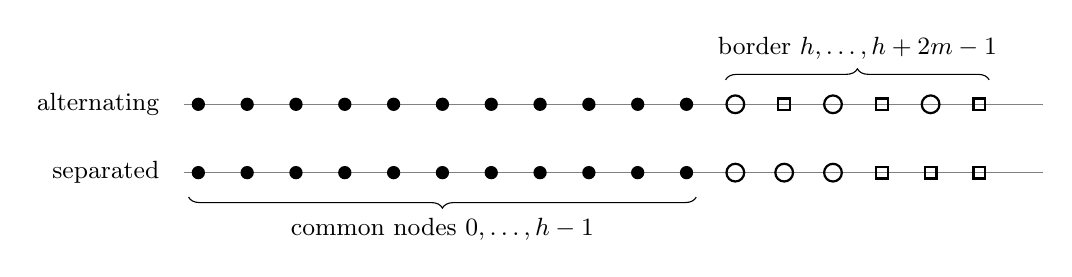
\begin{tikzpicture}[x=0.62cm,y=0.62cm]
  \foreach \yy/\lab in {1.4/alternating, 0/separated}{
    \node[anchor=east] at (-0.6,\yy) {\small\lab};
    \draw[gray] (-0.3,\yy) -- (17.3,\yy);
    \foreach \x in {0,...,10} {\fill (\x,\yy) circle (2.4pt);}
  }
  \foreach \x in {11,13,15}{\draw[thick] (\x,1.4) circle (3.2pt);}
  \foreach \x in {12,14,16}{\draw[thick] (\x-0.12,1.28) rectangle (\x+0.12,1.52);}
  \foreach \x in {11,12,13}{\draw[thick] (\x,0) circle (3.2pt);}
  \foreach \x in {14,15,16}{\draw[thick] (\x-0.12,-0.12) rectangle (\x+0.12,0.12);}
  \draw[decorate,decoration={brace,amplitude=4pt,mirror}] (-0.2,-0.5) -- (10.2,-0.5)
    node[midway,below=4pt] {\small common nodes $0,\dots,h-1$};
  \draw[decorate,decoration={brace,amplitude=4pt}] (10.8,1.9) -- (16.2,1.9)
    node[midway,above=4pt] {\small border $h,\dots,h+2m-1$};
\end{tikzpicture}
\caption{Schematic node geometries ($m=3$). Filled discs are common nodes, circles border rows,
squares border columns.}
\label{fig:geometries}
\end{figure}

\subsection{Status of the steps}\label{subsec:status}

\Cref{tab:status} gives the status of each step. \emph{Proved} means a complete proof, possibly
reviewed by an AI system; \emph{certified (AI-internal)} means a rigorous computation that was
recomputed, by implementations written separately from the original programs, in an internal
audit performed by an AI system (the \emph{AI-internal audit}); \emph{candidate} means a written
proof that has not been independently verified. A certified computation is only as good as the
statements that reduce the mathematics to it; these are listed in the table as separate steps.
No step has been checked by a human, and no AI review is independent certification. The open
points are listed in \cref{subsec:open-points}.

\begin{table}[ht]
\centering
\small
\begin{tabular}{@{}>{\raggedright\arraybackslash}p{0.34\textwidth}>{\raggedright\arraybackslash}p{0.20\textwidth}>{\raggedright\arraybackslash}p{0.36\textwidth}@{}}
\toprule
step & status & evidence\\
\midrule
separation identity (\cref{cor:separation}) & proved & AI-internal adversarial review; exact checks for $h\le64$\\
nonvanishing (\cref{prop:nonvanishing}) & candidate & no review; no rational roots for $h\le48$\\
entrywise bounds (\cref{lem:entry-bound}) & proved & elementary\\
polar congruences, nullspace bound (\cref{lem:two-layer}, \cref{prop:nullspace}) & candidate & checked in the AI-internal audit; finite tests up to $h=128$\\
profile bound and profile structure (\cref{lem:profile-bound}, \cref{lem:profile-structure}) & candidate & proofs written here, no review; affinity checked at five points of each cell\\
value of $\cA$ (\cref{prop:A-value}) & certified (AI-internal), given \cref{lem:profile-structure} & two exact implementations agree; the exact integration uses the breakpoints of \cref{lem:profile-structure}\\
prime number theorem bookkeeping (\cref{thm:arithmetic}) & candidate & standard; no review\\
contour representation, energy criterion (\cref{lem:contour}, \cref{prop:energy-criterion}) & candidate & inequality checked in the AI-internal audit\\
energy constants (\cref{prop:energy-certificate}) & certified (AI-internal) & ball arithmetic; the original fixed-point verifier gives a slightly weaker bound\\
final deduction (\cref{subsec:main-proof}) & proved & elementary; formalized in Lean conditionally on the estimates\\
\midrule
\cref{thm:main} & candidate & no human review\\
\bottomrule
\end{tabular}
\caption{Status of the steps of the proof.}
\label{tab:status}
\end{table}

\subsection{Notation and conventions}\label{subsec:notation}

Throughout, $k\in\{1,2,3,4\}$ and $s=k/5$; all logarithms are natural; implied constants in
$O(\cdot)$ and $o(\cdot)$ may depend on $k$ and on the rational number $X$ under consideration,
never on $h$, on a prime $p$ or on the deletion $I$; and asymptotic statements are as
$h\to\infty$ through $16\N$. \Cref{tab:notation} lists the notation used in more than one section.

\begin{table}[ht]
\centering
\small
\begin{tabular}{@{}>{\raggedright\arraybackslash}p{0.20\textwidth}>{\raggedright\arraybackslash}p{0.50\textwidth}>{\raggedright\arraybackslash}p{0.16\textwidth}@{}}
\toprule
symbol & meaning & defined in\\
\midrule
$F$, $\delta$ & $\psi(z+s)-\psi(z+\frac12)$, and $\delta(z)=F(z+1)-F(z)$ & \cref{subsec:function}\\
$f_x$, $d_x$ & $F(x)-F(0)$, $F'(x)-F'(0)$ for $x\in\Z_{\ge0}$ (rational) & \cref{subsec:function}\\
$h,m,n,N$ & $h\in16\N$, $m=h/16$, $n=h+m$, $N=h+2m$ & \cref{def:geometries}\\
$c$, $\lambda$ & border ratio $2m/h=\frac18$; $\lambda=n/h=\frac{17}{16}$ & \cref{def:geometries}\\
$\Nod,\Com,\Bor$ & all nodes $\{0,\dots,N-1\}$, common nodes $\{0,\dots,h-1\}$, border & \cref{def:geometries}\\
$\Row^\star,\Col^\star$ & row and column nodes, $\star\in\{\alt,\sep\}$ & \cref{def:geometries}\\
$I$, $n_I$ & deletion ($I\subseteq\Com$), size $n-\abs I$ of the pencil & \cref{def:geometries}\\
$M^\star_I(X)$, $P^\star_I(X)$ & L\"owner pencil and its determinant & \cref{def:pencil}\\
$g[x,y]$, $L_g(\Row,\Col)$ & divided differences of $g$, L\"owner matrix & \cref{subsec:partition}\\
$\Delta(S)$, $\omega_S$ & $\prod_{a<b}(x_b-x_a)>0$ and $\prod_{x\in S}(z-x)$ for $S=\{x_1<\dots<x_n\}\subset\R$; $\Delta(z)=\prod_{a<b}(z_b-z_a)$ for $z\in\C^n$ & \cref{subsec:andreief}\\
$\den r$, $v_p$, $e_p$, $\Zp$ & denominator of $r\in\Q$ ($\den0=1$), $p$-adic valuation, $e_p(r)=\max(0,-v_p(r))$, rationals with denominator prime to $p$ & \cref{sec:arithmetic}\\
$\kappa$, $V^\varepsilon_l$, $W^\varepsilon_l$ & root class of $p$ and polar values & \cref{subsec:polar}\\
$u$, $\gamma(t)$, $T(t)$ & the ratio $p/h$; numbers of common digits and of all digits of a fibre & \cref{subsec:profile}\\
$e_\kappa$, $\cA$ & profile and arithmetic constant & \cref{subsec:profile,subsec:integration}\\
$\nu$, $\mu$, $\Gamma$ & node measure, trial measure, contour & \cref{sec:decay}\\
$\pot\mu$, $I(\mu)$ & logarithmic potential and energy & \cref{subsec:energy-prelim}\\
$\cD_{\alt}$, $\cD_{\sep}$, $\cD^{*}_{\alt}$ & certified lower bounds for the decay rates of the two geometries (truncated decimals), and the certified rational bound & \cref{sec:decay}\\
\bottomrule
\end{tabular}
\caption{Notation.}
\small
\label{tab:notation}
\end{table}
